\documentclass[12pt,a4paper,oneside]{report}
\usepackage{indentfirst}
\usepackage{times}
\setlength\parindent{6ex}
\renewcommand{\baselinestretch}{1.50}\normalsize
\usepackage{anysize}
\marginsize{1.25in}{.75in}{1in}{1in}
\usepackage{graphics}
\usepackage{graphicx}
\usepackage{epsfig}
\usepackage[fleqn]{amsmath}
\usepackage{amsfonts}
\usepackage{textcomp}
\usepackage{graphicx}
\usepackage{float}
\usepackage{enumitem}
\usepackage{setspace}
\usepackage{fancyhdr}
\usepackage{truncate}
\usepackage{nomencl} 
\usepackage{acronym}
\usepackage{array}
\usepackage{caption}
\usepackage{cite}
\usepackage{subcaption}
\usepackage[overload]{textcase}
\usepackage{listings}
\renewcommand{\nomname}{List of Abbreviations}
\usepackage{makeidx}
\makeindex
\makenomenclature
\newcommand{\quotes}[1]{``#1''}
\usepackage{titlesec}
\titleformat{\chapter}[display]
{\normalfont\Large\bfseries\centering}
{\chaptertitlename\ \thechapter}{15pt}{\LARGE}
\titleformat{\section}{\large\bfseries}{\thesection}{1em}{}
\titleformat{\subsection}{\normalsize\bfseries}{\thesubsection}{1em}{}
\renewcommand{\chaptermark}[1]{\markboth{ \emph{#1}}{}}

\printnomenclature[5em]
\pagestyle{fancy}
%\headheight 1pt
	\renewcommand{\footrulewidth}{1.2pt}
\renewcommand{\headrulewidth}{1.2pt}
\rhead{\scriptsize {\leftmark}}

\lhead{\small{College of Engineering, Cherthala \;\;\;\;\;\;\;\;\;\;\;\;\;\;\;\;\;\;}}
\rfoot{\thepage}
\cfoot{\empty}
\lfoot{\small{Department of Computer Science \& Engineering}}
\renewcommand{\figurename}{Fig.}
\begin{document}
\renewcommand\bibname{References}
\begin{titlepage}
\begin{center}
\Large{\textbf{A SEMINAR REPORT ON}}\\
\vspace{.2 in}
\begin{singlespace}
\LARGE{\textbf{Jamstack}}\\
\end{singlespace}
\vspace{.2 in}
\Large{\textit{Submitted By }}\\
\Large{\textit{\textbf{AROMAL ANIL}}} \\
\textbf{Reg. No . CEC17CS018}\\
\Large{\textit{\textit{under the esteemed guidance of}}}\\
\Large{\textit{Mrs. Jisy Raju}}\\
\Large{\textit{Assistant Professor}}\\
\Large{\textit{Computer Science \& Engineering}}
\vspace{.05in}
\begin{figure}[h]
\begin{center}

\epsfig{width=1.5 in, file=logo.jpg}
\end{center}
\end{figure}
\begin{singlespace}
\large{\textbf{October 2020}}\\
\vspace{.2in}
\large{\textbf{DEPARTMENT OF COMPUTER SCIENCE AND ENGINEERING\\COLLEGE OF ENGINEERING,CHERTHALA\\ PALLIPPURAM P O, ALAPPUZHA-688541, \\PHONE: 0478 2553416, FAX: 0478 2552714\\http://www.cectl.ac.in}}
\end{singlespace}
\end{center}
\end{titlepage}

\begin{titlepage}
\begin{center}

\large{\textbf{A SEMINAR REPORT ON}}\\
\begin{singlespace}
\LARGE{\textbf{Web of Things}}\\
\end{singlespace}


\Large{\textit{Submitted By }}\\
\Large{\textit{\textbf{AROMAL ANIL}     (\textbf{Reg. No . CEC17CS018})}}\\
\Large{\textit{\textit{under the esteemed guidance of}}}\\
\Large{\textit{Mrs. Jisy Raju}}\\
\begin{singlespace}
\large{\textit{In partial fulfillment of the requirements for the award of the degree}\\
\large{ \textit{of}}\\
\large{\textit{Bachelor of Technology} }\\
\large{\textit{in}}\\
\large{\textit{Computer Science and Engineering}}\\
\large{\textit{of}}\\
\large{\textit{Cochin University Of Science And Technology}}}\\
\end{singlespace}
\begin{figure}[h]
\begin{center}

\epsfig{width=1.5 in, file=logo.jpg}
\end{center}
\end{figure}
\begin{singlespace}

\Large{\textbf{October 2020\\Department of Computer Science and Engineering\\College of Engineering, Pallippuram P O, Cherthala, Alappuzha Pin: 688541, \\Phone: 0478 2553416, Fax: 0478 2552714\\http://www.cectl.ac.in}}
\end{singlespace}
\end{center}
\end{titlepage}


\begin{titlepage}
\begin{center}

\large{\textbf{DEPARTMENT OF COMPUTER SCIENCE \& ENGINEERING}}\\
\large{\textbf{COLLEGE OF ENGINEERING CHERTHALA\\ALAPPUZHA-688541}}\\
\end{center}
\begin{figure}[h]
\begin{center}

\epsfig{width=1.5in, file=logo.jpg}
\end{center}
\end{figure}
\begin{center}
\large{\textbf{C E R T I F I C A T E}}\\
\end{center}
\begin{spacing}{1.5}
This is to certify that, the seminar report titled  \textbf{\textit{ JAMSTACK}} is a bonafide record of the \textbf{CS405 SEMINAR} presented by \textbf{AROMAL ANIL} (Reg.No.CEC17CS018), Seventh Semester B. Tech. Computer Science \& Engineering  student,  under our guidance and supervision, in partial fulfillment of the requirements for the award of the degree, \textbf{B. Tech. Computer Science  \& Engineering } of \textbf{APJ Abdul Kalam Technological University}.
\end{spacing}
\begin{tabbing}
xxxxxxxxxxxxxxxxxxxxxxxxxxxxxxxxxxxxxx\= xxxxxxxxxxxxxxxxxxxx\= \kill
\hspace{.15in}{\bf Guide} \>\hspace{-.7in}{\bf Co-ordinator}\hspace{1.32in}{\bf  HoD  } \\
\end{tabbing}
\begin{tabbing}
xxxxxxxxxxxxxxxxxxxxxxxxxxxxxxxxxxxxxx\= xxxxxxxxxxxxxxxxxx\= \kill
%\vspace{0.3in}\\
\hspace{.15in}{\bf{Mrs. Jisy Raju}}   \>\hspace{-.7in}{\bf Mrs. Janu R Panicker} \hspace{.65 in}{\bf Dr. Priya S}\\
\hspace{.15in}Assistant Professor    \>\hspace{-.7in}Assistant Professor\>\hspace{.06in} Professor\\
\hspace{.1in} Computer Science \& Engg.    \>\hspace{-.75in}    Computer Science \& Engg. \>\hspace{.03in}    Computer Science \& Engg.\\

\end{tabbing}
\end{titlepage}


\renewcommand*\thesection{\thechapter.\arabic{section}}
%\pagenumbering{arabic}
%\addtocounter{page}{4}

\begin{titlepage}
\pagenumbering{roman}
%\addtocounter{page}{4}
\setcounter{page}{4}
\section*{\begin{center} \Large{ACKNOWLEDGEMENT }\end{center}}

\thispagestyle{plain}


%{$\;\;\;\:$}
\par
This work would not have been possible without the support of many people.
First and the foremost, I give thanks to Almighty God who gave me the inner strength, resource and ability to complete my seminar successfully.
\par
I would like to thank \textbf{Dr. Mini M G}, The Principal, who has provided with the best facilities and atmosphere for the seminar completion and presentation. I would also like to thank HoD \textbf{Dr. Priya S} (Professor, Computer Science and Engineering) and my seminar guide \textbf{Mrs.Jisy Raju} (Assistant Professor, Computer Science and Engineering), my seminar coordinator \textbf{Mrs. Janu R Panicker} (Assistant Professor, Computer Science and Engineering) for the help extended and also for the encouragement and support given to me while doing the seminar.
\par
I would like to thank my dear friends for extending their cooperation and encouragement throughout the seminar work, without which I would never have completed the seminar this well. Thank you all for your love and also for being very understanding. 

\end{titlepage}
\newpage

\section*{\begin{center}\Large ABSTRACT\end{center}}
\thispagestyle{plain}
\setcounter{page}{5}
\par
\hspace{0.1in}
Jamstack is a hot topic in the developer community. It is a methodology to build fast, reliable and secure web projects. Jamstack stands for JavaScript, API \& Markup. The basic idea of Jamstack is to bring dynamic capabilities to static websites using JavaScript, APIs \& Modern frontend frameworks.\\

\pre
The emergence of many Modern frontend frameworks and the introduction of Node.js made it easy for the frontend developers to implement many backend functionalities. This lead to the introduction of a frontend-centric tech-stack in web community.\\

\pre
The Static site generators like Hugo, Gatsby, Next.js etc. \& Headless CMS like Strapi, Contentful etc also increased the popularity of Jamstack. Due to the speed, reliable, cost efficient \& developer friendly nature Jamstack is now one of the popular tech-stacks in the Web community.
\\
\\\hspace{-.43in} 
\textbf{Keywords--} \textit{\textbf{Jamstack, Website Development, JavaScript, API, Markup }}

%\pagenumbering{arabic}
%\setcounter{page}{5}
\tableofcontents
%\pagenumbering{arabic}
%\listoftables
\listoffigures
%\listoftables



%\renewcommand*\thesection{\thechapter.\arabic{section}}
\newpage
\pagestyle{fancy}
\headheight 26pt
\renewcommand{\footrulewidth}{1.2pt}
\renewcommand{\headrulewidth}{1.2pt}
\rhead{\scriptsize {\leftmark}}
\lhead{\small{College of Engineering, Cherthala \;\;\;\;\;\;\;\;\;\;\;\;\;\;\;\;\;\;}}
\rfoot{\thepage}
\cfoot{\empty}
\lfoot{\small{Department of Computer Science \& Engineering}}
\pagenumbering{arabic}
\chapter{INTRODUCTION}
\label{intro}
%\pagenumbering{arabic}
%\setcounter{page}{1}
%\hspace{0.1in}

{
``\textit{A modern web development architecture based on client-side JavaScript, reusable APIs, and prebuilt Markup}''\\
\rightline{ --- Mathias Biilmann (CEO & Co-founder of Netlify)}}\\
\par
Jamstack is a new approach to faster, more secure websites. Jamstack stands for JavaScript, API \& Markup. The term `Jamstack' was first coined in the year 2015 by Mathias Biilmann.Jamstack is a term for a common web application architecture in which a web app consists primarily of pre-rendered, static HTML that relies on client-side APIs and JavaScript to provide interactive elements.\cite{official}

\par
Jamstack can be also described as Static sites with Dynamic Capabilities. The basic concept of Jamstack to serve static contents to the user on request \& providing Dynamic abilities to it using APIs.
\par
The ever growing community of Jamstack has introduced many Static-site generators, Headless CMS and Jamstack Hosts over time. 

\begin{figure}
    \centering
    
\includegraphics[scale=.2]{images/Jamstack-logo.png}
    \caption{Jamstack Logo\cite{official}}
\end{figure}

\grap

\chapter{LEGACY WEB}

\section{Other Tech Stacks}
\pre 
Before the introduction of Jamstack there where many other tech-stacks used in web development. Some of them are: 

\subsection{LAMP}
\begin{figure}[H]
    \centering
    
\includegraphics[scale=.15]{images/lamp.jpg}
    \caption{LAMP Stack\cite{lamp}}
\end{figure}

\par 
Linux based web servers consist of four software components. These components, arranged in layers supporting one another, make up the software stack. Websites and Web Applications run on top of this underlying stack. The common software components that make up a traditional LAMP stack are\cite{lamp}:
\begin{itemize}
\item \textbf{Linux}: The operating system (OS) makes up our first layer. Linux sets the foundation for the stack model. All other layers run on top of this layer.
\item \textbf{Apache}: The second layer consists of web server software, typically Apache Web Server. This layer resides on top of the Linux layer. Web servers are responsible for translating from web browsers to their correct website.
\item \textbf{MySQL}: Our third layer is where databases live. MySQL stores details that can be queried by scripting to construct a website. MySQL usually sits on top of the Linux layer alongside Apache/layer 2. In high end configurations, MySQL can be off loaded to a separate host server.
\item \textbf{PHP}: Sitting on top of them all is our fourth and final layer. The scripting layer consists of PHP and/or other similar web programming languages. Websites and Web Applications run within this layer.
\end{itemize}

\subsection{MEAN}

\begin{figure}[H]
    \centering
    
\includegraphics[scale=.7]{images/mean.png}
    \caption{MEAN Stack\cite{mean}}
\end{figure}

\par 
MEAN is a full-stack JavaScript solution that helps you build fast, robust, and maintainable production web applications using MongoDB, Express, AngularJS, and Node.js.\cite{mean}

\subsection{MERN}

\begin{figure}[H]
    \centering
    
\includegraphics[scale=.25]{images/mern.png}
    \caption{MERN Stack\cite{mern}}
\end{figure}

\par 
MERN Stack: MERN Stack is a JavaScript Stack that is used for easier and faster deployment of full-stack web applications. MERN Stack comprises of 4 technologies namely: MongoDB, Express, React and Node.js. It is designed to make the development process smoother and easier.
Each of these 4 powerful technologies provides an end-to-end framework for the developers to work in and each of these technologies play a big part in the development of web applications\cite{mern}.

\section{Problem with these Tech-stacks}

\pre 
These all tech stacks have advantages \& disadvantages of their own. But some of the common issues in these stacks are:
\begin{enumerate}
\item \textbf{Backend-Centric} : All these stacks are backend-centric and all the components are run in the backend.
\item \textbf{Server Side Rendering} : In all of these tech stacks the web server will render the web page based on the request received, by fetching the necessary data from the database.
\item \textbf{Costly} : Each of these tech stacks require a dedicated server to run. It is hard to run these on a server less environment.
\end{enumerate}




\chapter{JAMSTACK}
\section{What is Jamstack ?}
Jamstack stands for JavaScript, API \& Markup. It is an architecture designed to make the web faster, more secure, and easier to scale. It is not a programming language or any form of tool. But, it is builds on many of the tools and workflows which developers love, and which bring maximum productivity.

\subsection{JavaScript}
\begin{figure}[H]
    \centering
    
\includegraphics[scale=.2]{images/javascript.png}
    \caption{JavaScript\cite{js}}
\end{figure}
\par 
JavaScript is a dynamic computer programming language. It is lightweight and most commonly used as a part of web pages, whose implementations allow client-side script to interact with the user and make dynamic pages. It is an interpreted programming language with object-oriented capabilities.
\par
JavaScript is the part which gives dynamic functionalities to the served static site. Whether it be simple button interaction or data fetching, JavaScript handles it all with ease.. There is no restriction on which framework or library you must use. The JavaScript will be running entirely on the client.

\subsection{API}
\begin{figure}[H]
    \centering
    
\includegraphics[scale=.2]{images/api.png}
    \caption{API\cite{api}}
\end{figure}
\par 
An application programming interface is a computing interface which defines interactions between multiple software intermediaries. It defines the kinds of calls or requests that can be made, how to make them, the data formats that should be used, the conventions to follow, etc.
\par 
The APIs used in Jamstack are server APIs. In Jamstack Server side operations to be performed are abstracted into reusable APIs and are accessed over HTTPS with JavaScript. These can be third party services or your custom function.

\subsection{Markup}
\begin{figure}[H]
    \centering
    
\includegraphics[scale=.2]{images/html.png}
    \caption{Hypertext Markup Language\cite{html}}
\end{figure}
\par 
A markup language is a system for annotating a document in a way that is syntactically distinguishable from the text, meaning when the document is processed for display, the markup language is not shown, and is only used to format the text.
\par 
Websites are served as static HTML files. Templated markup should be prebuilt at build time, usually using a site generator for content sites, or a build tool for web apps.
\par 
Markdown and HTML are the common markup languages used in Jamstack. HTML is the markup language with which the web is made, so the generated static sites will always be HTML. But due to simple syntax and readability often the web contents are saved as Markdown files \& then later converted or processed to HTML using static site generators.

\chapter{WORKFLOW}
\section{Jamstack Workflow}
\begin{figure}[H]
    \centering
    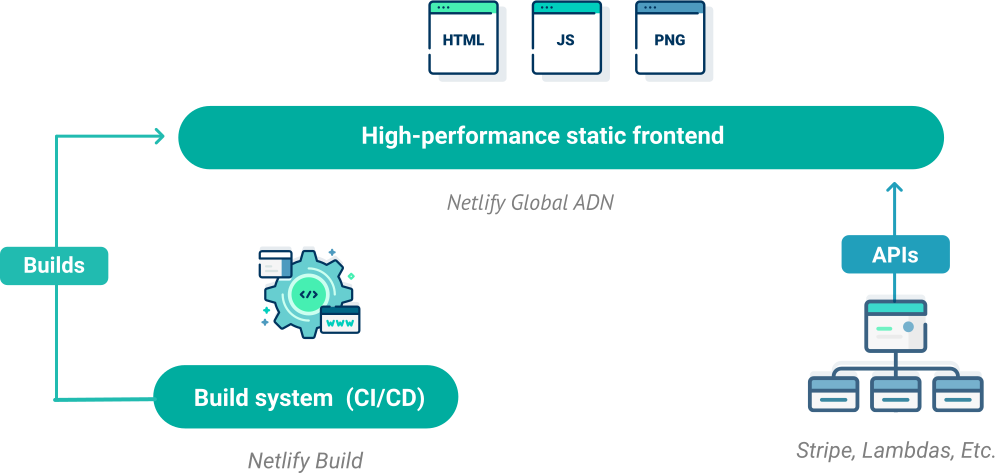
\includegraphics[scale=.3]{images/how-it-works.png}
    \caption{Hypertext Markup Language\cite{wjam}}
\end{figure}
\par 
The basic workflow of Jamstack website is as follows
\subsection{Development \& Publishing}
\par
The Developer publishes the static sites to the CDN or any other hosting option. This static sites can be coded from scratch or can be generated using any static site generators like Hugo, Gatsby etc during the build time.
\subsection{Serving web-pages}
\par 
The web-pages are served to the user upon request directly from the CDN or the location where static contents are hosted. The page served can be plain HTML web-pages or Single Page Applications like Hydrated React apps.
\subsection{JavaScript Execution}
\par 
After the static HTML is rendered in the browser, JavaScript kicks in. In the case of apps made with React, the content is rendered in the client side using JavaScript. In the case of ordinary web-pages, JavaScript adds interactivity to it. The JavaScript listens for state changes and performs the necessary actions as per instructions.
\subsection{Use of API}
\par 
For any dynamic content, or sever-side needs, Jamstack rely on APIs. JavaScript calls the API end point when needed and updates the web-page according to the received response.
\par 
The API can be any self-maintained API or third-party solutions. Cloudinary, Algolia, Netlify-Forms etc are some of the third party API solutions each providing different functionalities.




\chapter{JAMSTACK TIMELINE}
Let’s take a quick journey back in time with a year-by-year view of the rise of the Jamstack. It should clarify where it’s at right now and where it’s going \cite{snip}.

\section{Important Events in Jamstack}

\begin{itemize}
\item  \textbf{2015} : Static sites are slowly making a comeback from the ruins of the web’s early years. The first CMS-deniers starts to emerge.
\item \textbf{2016} : In the developer community, backlash occurs. Static sites are not accepted by many, the argument raised was they lack too many features to build anything other than blogs. In the meantime though, a small group of developers is coining the “Jamstack” and slowly promoting its principles in modern dev circles.
\item \textbf{2017} : The year Jamstack really comes to life, for a somewhat niche community. Static sites aren't “static” anymore. This modern web revolution provides all the features you need to build “hyper-dynamic” sites \& apps. Sequoia Capital, Mailchimp \& Red Bull are a few of the first big enterprises to build Jamstack projects.
\item \textbf{2018} : The developers started learning \&  wildly adapting Jamstack. The paradigm makes a mainstream breakthrough with more \& more people talking about it. Substantial funding is announced for tools like Gatsby, Netlify, Contentful, etc. The first Jamstack\--conf takes place.

\begin{figure}[H]
    \centering
    
\includegraphics[scale=.2]{images/jam-conf-2018.jpg}
    \caption{JAMstack Conf 2018\cite{conf}}
\end{figure}

\item  \textbf{2019} : The year of maturity \& accessibility. The Jamstack isn’t a niche community anymore. Most frontend developers hear about it and many start looking into it. With the likes of Stackbit, the Jamstack opens its doors to less technical users. The rise of serverless functions is also huge for bringing more backend functionalities to frontend-centric projects.
\item \textbf{2020} : With a new decade on the horizon, there’s nothing indicating a decline in the Jamstack’s adoption. If services and APIs in the ecosystem continue to prove viable and profitable, we’ll see more important players embracing the idea, increasing adoption even more. The New Dynamic brought legit concerns about having too much options in the ecosystem in its first newsletter of the year. 
\end{itemize}

\chapter{JAMSTACK VS TRADITIONAL WEB}

\section{Workflow Comparison}

\begin{figure}[H]
    \centering
    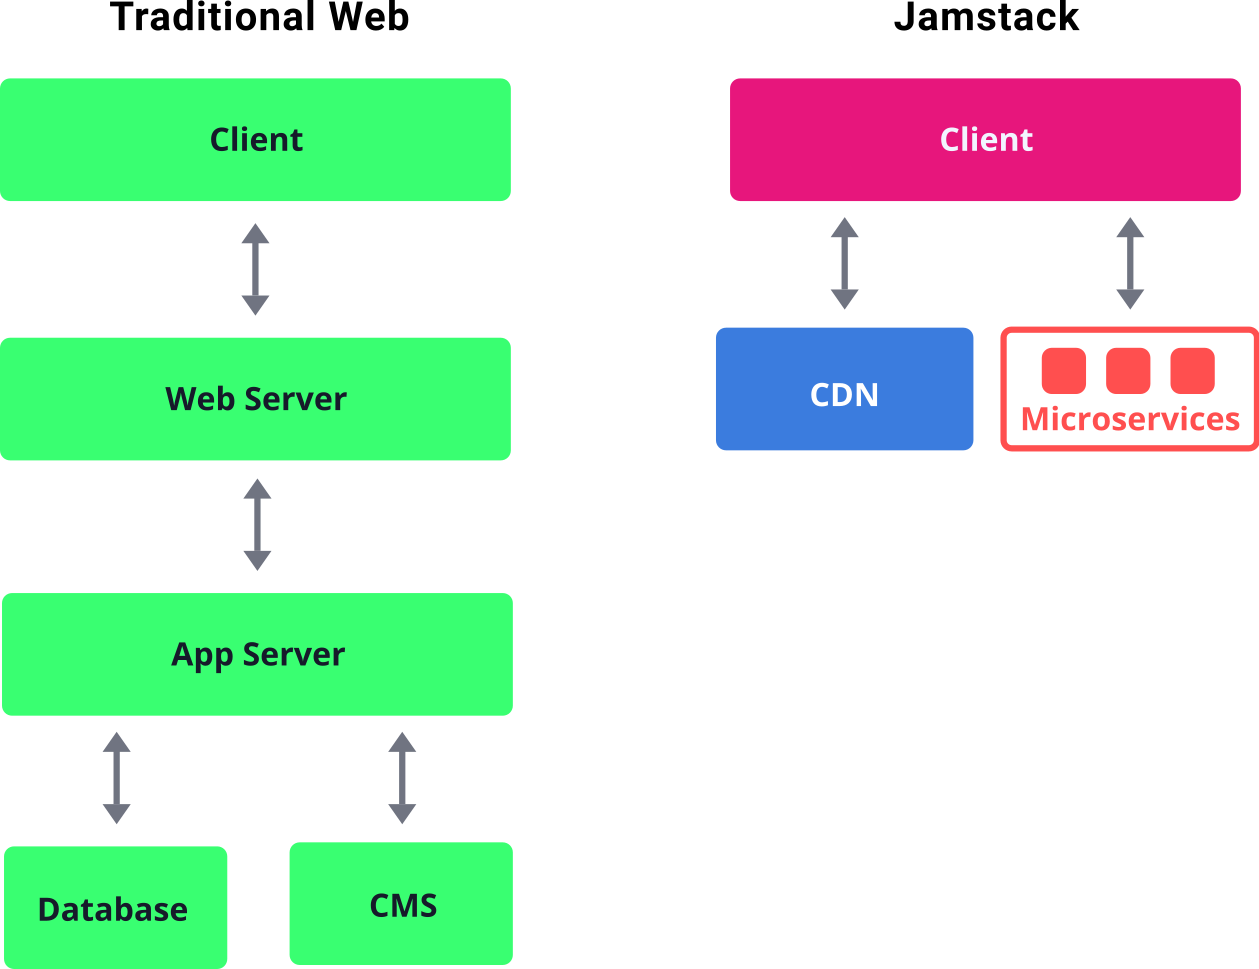
\includegraphics[scale=1]{images/comparison.png}
    \caption{Traditional Web vs Jamstack\cite{official}}
\end{figure}

\subsection{Traditional Workflow}
\begin{itemize}
    \item Building and hosting are coupled.
    \item A user requests a page. The file gets processed and served following a (long) series of interaction between a database, backend code, server, browser, and layers of caching.
    \item  Core updates are pushed to production servers, often through FTP. Database must be maintained or updated.
    \item  Content updates are pushed through traditional CMS, like WordPress or Drupal.
\end{itemize}

\subsection{Jamstack Workflow}
\begin{itemize}
\item Building and hosting are decoupled.
\item A user requests a page. The file is already compiled and gets directly served to the browser from a CDN.
\item Core updates are pushed through Git; the site gets re-built entirely via modern build tools like static site generators.
\item Content updates are pushed through Git or a static site CMS.
\end{itemize}


\chapter{ADVANTAGES OF JAMSTACK}
So we have seen whats Jamstack is \& How it works. But, what makes a Jamstack app so great? Let's take a look
\section{AWS Well-Architected Framework}
\par 
Even though Jamstack is not a framework on it's own, every app made using Jamstack methodology satisfy most if not all of the 5 pillars of the AWS Well-Architected Framework. 

\begin{figure}[H]
    \centering
    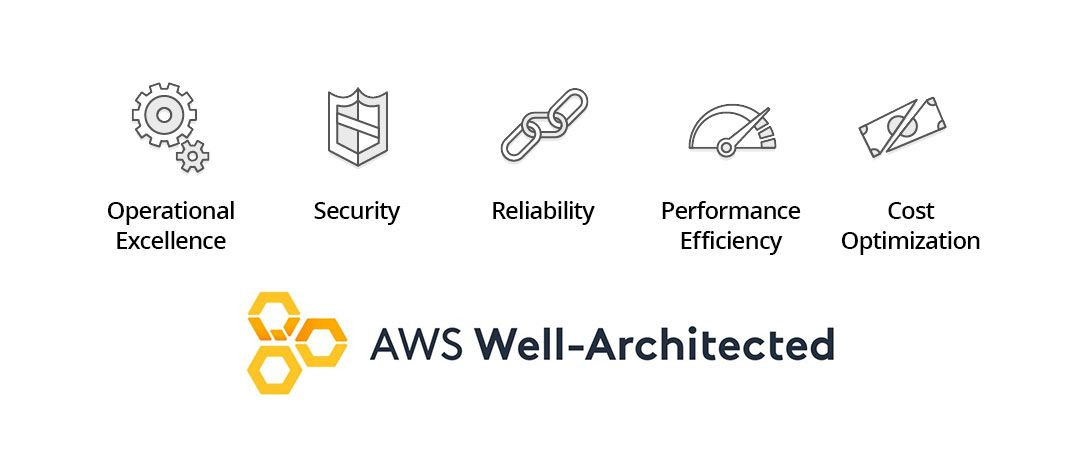
\includegraphics[scale=.35]{images/aws-well-architected-framework.jpg}
    \caption{Characters of AWS Well-Architected Framework\cite{fcc2}}
\end{figure}

\par 
The core concepts that AWS considers to deliver fast, secure, high-performing, resilient, and efficient infrastructure are :

\begin{itemize}
\item Operational Excellence.
\item Security
\item Reliability
\item Performance Efficiency
\item Cost Optimisation
\end{itemize}

\section{Fast Performance}
\par
When it comes to minimizing the time of load, nothing beats pre-built files served over a CDN. Jamstack sites are super fast because the HTML is already generated during deploy time and just served via CDN without any interference or backend delay. In many cases the the page of the app are served as just plain HTML ``as is'' or with some type of client side hydration like you’d see with React.

\par 
The static sites uploaded to the CDN generally don't change very often, this gives the opportunity to duplicate and save the static files globally across many proxy servers of the CDN. So that when a user request a web-page it is served from the nearest proxy server. Many CDN providers offer this service.

\begin{figure}[H]
    \centering
    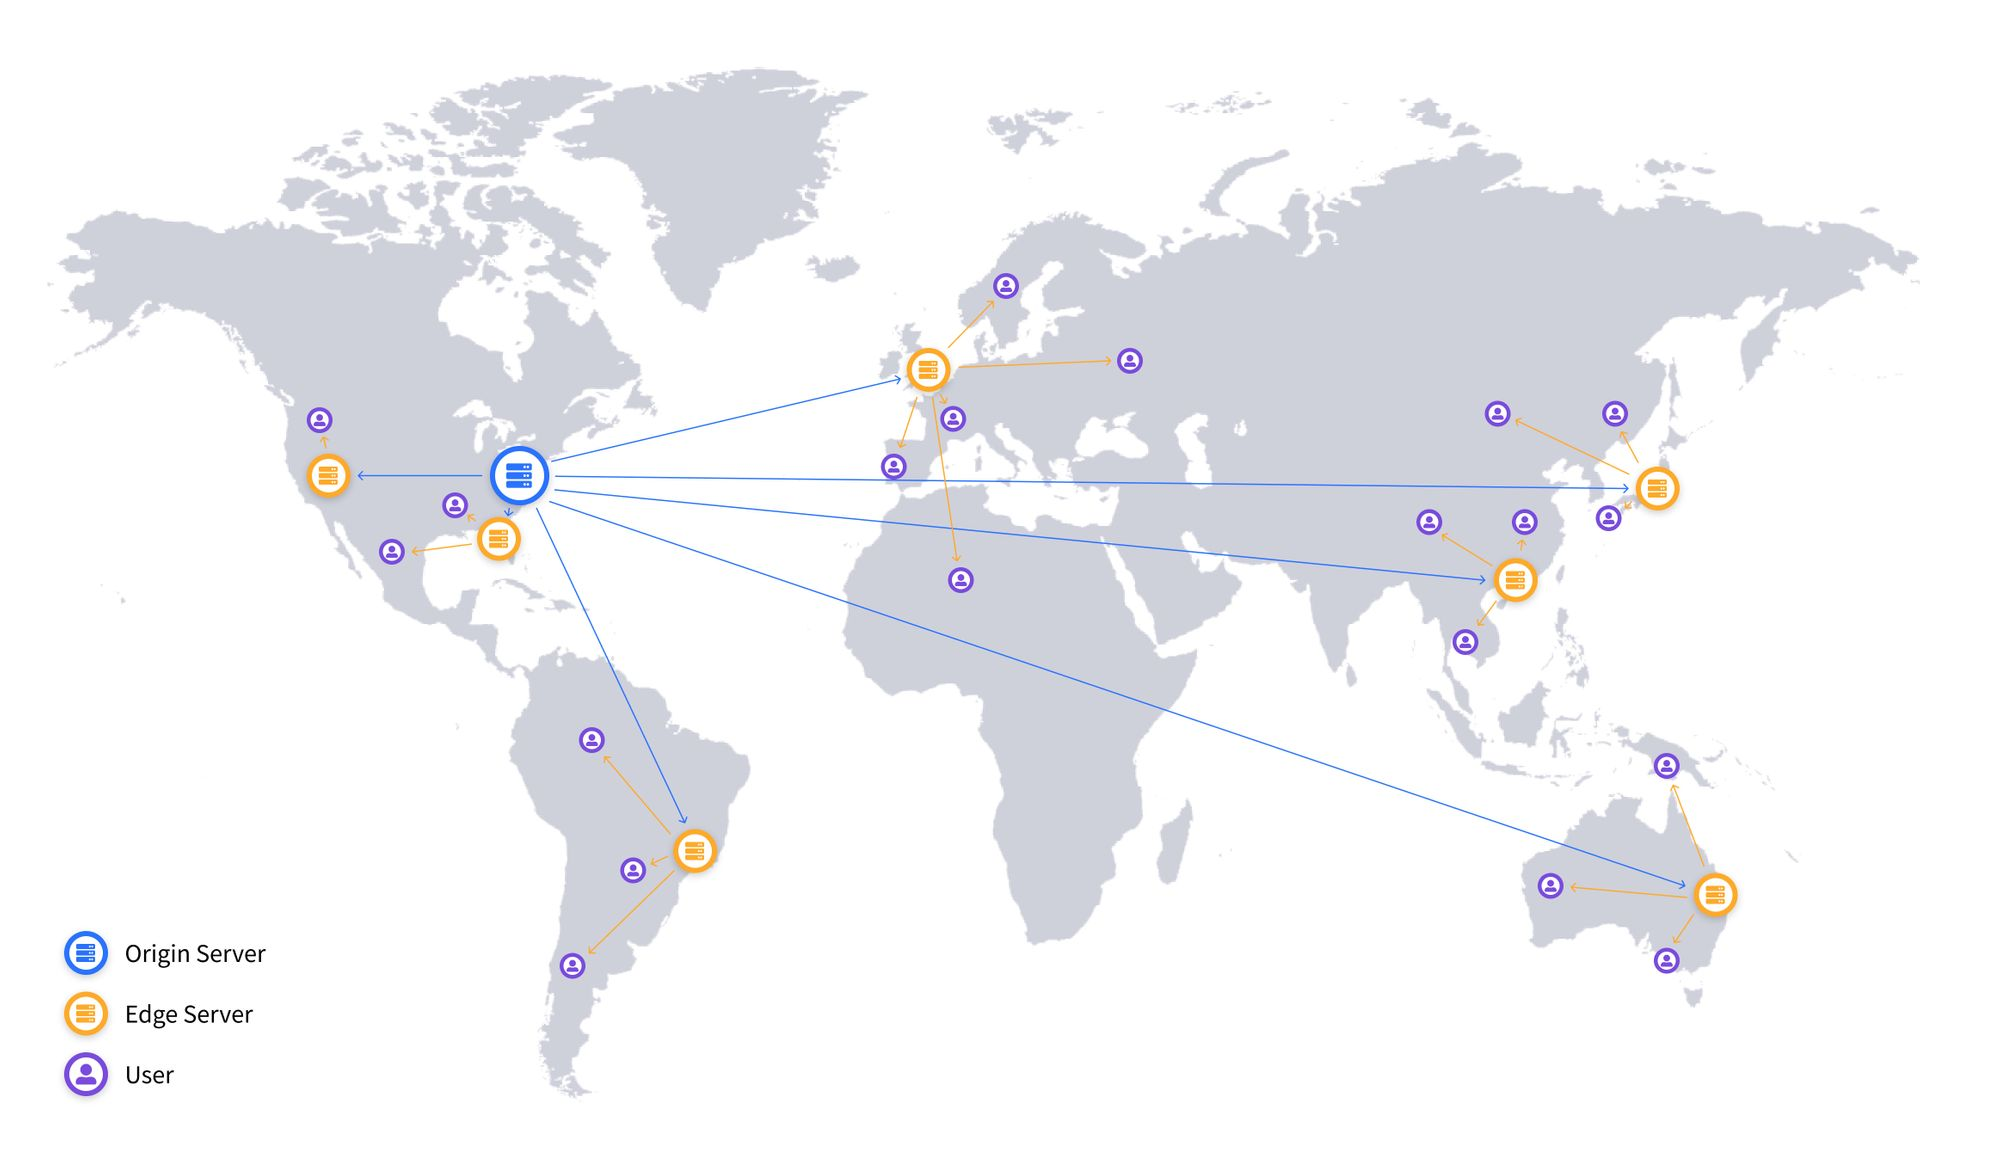
\includegraphics[scale=.18]{images/cdn-distribution-map.jpg}
    \caption{CDN Distribution Map\cite{fcc2}}
\end{figure}

\par 
Since the app need not to be rendered on the sever for each request, this eliminates a lot of delay in serving the web-page.

\section{High security}

\par 
Doubling down on the lack of server that you have to personally maintain, you don’t really need to worry as much about locking down ways for people to intrude.

\par
Instead, you'll need to focus mostly on permissions to lock down private content and assure your users that their personal information isn't publicly available.

\par
Everything works via an API and hence there are no database or security breaches. With server-side processes abstracted into micro service APIs, surface areas for attacks are reduced and so your site becomes highly secured.

\begin{figure}[H]
    \centering
    
\includegraphics[scale=.3]{images/apis.png}
    \caption{Available API Services\cite{snip}}
\end{figure}

\section{Low Cost}

\par 
More often than not, Jamstack sites are going to run cheaper than their server side counterparts. Hosting static assets is cheap and now the same page can being served at the same rate.

\begin{figure}[H]
    \centering
    
\includegraphics[scale=.3]{images/netlify.png}
    \caption{Jamstack sites  can be hosted free on Netlify\cite{netjam}}
\end{figure}

\par 
Since no Server side rendering is involved, it reduces the load on the server, and if we compare a Jamstack API server with other counterparts, Jamstack server will be cheaper in most cases.

\par 
Jamstack sites only contain just a few files with minimal sizes that can be served anywhere. Scaling is a matter of serving those files somewhere else or via CDNs.

\section{Excellent Developer Experience}
\par 
The overall experience of developing and maintaining apps relies on how several app components of the underlying architecture work together. Loose coupling along with the advantage of having third-party services perform the cumbersome, labor-intensive tasks make for a smooth developer experience, freeing you up to focus on your app’s business logic and other important issues.

\begin{figure}[H]
    \centering
    
\includegraphics[scale=.22]{images/happy-developer.png}
    \caption{Happy Developers\cite{happy}}
\end{figure}

\chapter{CONCEPTS \& TOOLS}
This chapter introduces some of the common concepts \& tools used widely across Jamstack ecosystem.
\section{Concepts}
\subsection{Decoupling}
\par 
Decoupling is the process of creating a clean separation between systems or services. By decoupling the services needed to operate a site, each component part can become easier to reason about, can by independently swapped out or upgraded, and can be designated the purvue of dedicated specialists either within an organisation, or as a third party.
\subsection{Pre-Rendering}
\par
With Jamstack, the entire front end is prebuilt into highly optimized static pages and assets during a build process. This process of pre-rending results in sites which can be served directly from a CDN, reducing the cost, complexity and risk, of dynamic servers as critical infrastructure.
\par
With so many popular tools for generating sites, like Gatsby, Hugo, Jekyll, Eleventy, NextJS, and very many more, many web developers are already familiar with the tools needed to become productive Jamstack developers.

\subsection{Git Based Workflow}
\par 
With a Jamstack project, anyone should be able to do a git clone, install any needed dependencies with a standard procedure (like npm install), and be ready to run the full project locally. No databases to clone, no complex installs. This reduces contributor friction, and also simplifies staging and testing workflows.

\section{Tools}
\subsection{Static Site Generators}
\par 
Think of a static site generator as a script which takes in data, content and templates, processes them, and outputs a folder full of all the resultant pages and assets.

\par 
The greatest difference between a static site generator and a traditional web application stack, is that instead of waiting until a page is requested and then generating its view on demand each time, a static site generator does this in advance so that the view is ready to serve ahead of time. And it does so for every possible view of a site at build time\cite{official}.

\par
Some of the popular static site generators are Gatsby,Next.js,Hugo,Jekyll etc.

\subsection{Headless CMS}
\par 
A headless CMS is a back-end only content management system (CMS) built from the ground up as a content repository that makes content accessible via a RESTful API for display on any device.

\par 
The term “headless” comes from the concept of chopping the “head” (the front end, i.e. the website) off the “body” (the back end, i.e. the content repository). A headless CMS remains with an interface to add content and a RESTful API (JSON, XML) to deliver content wherever you need it. Due to this approach, a headless CMS does not care about how and where your content gets displayed. A headless CMS has only one focus: storing and delivering structured content.


\chapter*{GLOSSARY}

\begin{itemize}[leftmargin=.5in, label={}]
    \item{\textbf{API}: Application Programming Interface}
    \item{\textbf{HTTP}: Hyper Text Transfer Protocol}
    \item{\textbf{JS}: JavaScript}
    \item{\textbf{JSON}: JavaScript Object Notation}
    \item{\textbf{REST}: Representational State Transfer}
    \item{\textbf{SaaS}: Software As A Service}
    \item{\textbf{SSR}: Server Side Rendering}
\end{itemize}
  

%\chapter{REFERENCES}
\renewcommand{\bibname}{\uppercase{REFERENCES}}
\begin{thebibliography}{999}
\addcontentsline{toc}{chapter}{\hspace{0.19in} REFERENCES}

\bibitem{official}{\textbf{Jamstack Official Website}}\\https://jamstack.org/

\bibitem{wtf}{\textbf{JAMstack WTF}}\\https://jamstack.wtf/

\bibitem{fcc1}{\textbf{An introduction to the JAMstack: the architecture of the modern web}}\\https://www.freecodecamp.org/news/an-introduction-to-the-jamstack-the-architecture-of-the-modern-web-c4a0d128d9ca/

\bibitem{fcc2}{\textbf{What is the JAMstack and how do I get started?}}\\https://www.freecodecamp.org/news/what-is-the-jamstack-and-how-do-i-host-my-website-on-it/

\bibitem{netjam}{\textbf{Next.js + Netlify}}\\https://medium.com/@azizhk/next-js-netlify-c246ea070ae2

\bibitem{wjam} {\textbf{Welcome to the Jamstack}}\\https://www.netlify.com/jamstack/

\bibitem{snip}{\textbf{New to Jamstack? Everything You Need to Know to Get Started}}\\
https://snipcart.com/blog/jamstack

\bibitem{html}\textbf{HTML logo}\\
https://www.w3.org/html/logo/

\bibitem{js}\textbf{JavaScipt Logo}\\
https://commons.wikimedia.org/wiki/File:JavaScript-logo.png

\bibitem{api}\textbf{API Logo}\\
https://www.pngegg.com/en/png-dqpxs

\bibitem{happy}\textbf{How to Keep Your Developer Team Happy: Lead Dev New York 2019}\\
https://arc.dev/blog/happy-developers-7zr5xar1zs

\bibitem{conf}\textbf{Reflecting on London’s first JAMstack conference}\\
https://dev.to/philhawksworth/reflecting-on-london-s-first-jamstack-conference-13e9

\bibitem{lamp}\textbf{Web Development on LAMP Stack}\\
https://dreamlogic.io/expertise-lamp.html

\bibitem{mean}\textbf{Owebest Mean Stack Development}
https://www.owebest.com/mean-stack

\bibitem{mern}\textbf{MERN-logo}\\
https://commons.wikimedia.org/wiki/File:MERN-logo.png


\end{thebibliography}

\end{document}